%%%%%%%%%%%%%%%%%%%%%%%%%%%%%%%%%%%%%%%%%%%%%%%%%%
%% Bachelor's & Master's Thesis Template        %%
%% Copyleft by Dawid Weiss & Marta Szachniuk    %%
%% Faculty of Computing and Telecommunication   %%
%% Poznan University of Technology, 2020        %%
%%%%%%%%%%%%%%%%%%%%%%%%%%%%%%%%%%%%%%%%%%%%%%%%%%


\documentclass[10pt,a4paper,english,thesis]{dcsbook}

\usepackage[utf8]{inputenc}
\usepackage{babel}
\usepackage{listings}
\setcounter{secnumdepth}{4}
\setcounter{tocdepth}{3}

\usepackage{hyperref}
\usepackage{xcolor}
\hypersetup{
   colorlinks=false,
   %  colorlinks,
   %  citecolor=black,
   %  filecolor=black,
   %  linkcolor=black,
   %  urlcolor=black,
}

\captionsetup{justification=centering}

\begin{document}

%--------------------------------------
% Strona tytułowa
%--------------------------------------

\author{Pierwszy autor pracy}
\title{Temat pracy dyplomowej}
\supervisor{prof.~dr hab.~inż.~Imię Nazwisko}
\date{2020}
\maketitle
\frontmatter

% debug
% \cleardoublepage % Zaczynamy od nieparzystej strony

%--------------------------------------
% Miejsce na kartę pracy dyplomowej
%--------------------------------------

\thispagestyle{empty}\vspace*{\fill}%
\begin{center}Tutaj będzie karta pracy dyplomowej;\\oryginał wstawiamy do wersji dla archiwum PP, w pozostałych kopiach wstawiamy ksero.\end{center}%
\vfill\cleardoublepage%

%--------------------------------------
% Spis treści
%--------------------------------------

\tableofcontents{}
\mainmatter

% debug
% \cleardoublepage % Zaczynamy od nieparzystej strony

%--------------------------------------
% Rozdziały
%--------------------------------------

\chapter{Introduction}

\section{Motivation}

\section{Objective and scope of research}

\section{Structure of thesis}

\chapter{Serverless computing}

\begin{itemize}
    \item Martin Fowler - https://martinfowler.com/articles/serverless.html
    \item Mike Roberts (same author as above) - https://www.symphonia.io/what-is-serverless.pdf
    \item Cloud Native Computing Foundation - https://github.com/cncf/wg-serverless/tree/master/whitepapers/serverless-overview 
    \item Serverless Inc - https://serverless.github.io/guide/
    \item Cloud Programming Simplified: A Berkeley View on Serverless Computing - https://arxiv.org/pdf/1902.03383.pdf
    \item Serverless Computing: A Survey of Opportunities, Challenges and Applications - https://arxiv.org/pdf/1911.01296.pdf
    \item Serverless architecture with AWS Lambda - https://d1.awsstatic.com/whitepapers/serverless-architectures-with-aws-lambda.pdf
    \item Examples - AWS Serverless Applications Lens - https://docs.aws.amazon.com/wellarchitected/latest/serverless-applications-lens/wellarchitected-serverless-applications-lens.pdf
    \item Examples - https://www.youtube.com/playlist?list=PLhr1KZpdzukdeX8mQ2qO73bg6UKQHYsHb
\end{itemize}

\section*{Origins}

Around 15 years ago companies were entirely responsible for managing servers for their server-side applications \cite{RobertsChapin2017}. In 2006 Amazon announced the launch of Elastic Compute Cloud (EC2) that changed the way of thinking about that and enabled people to outsource overhead of initializing, managing and provisioning machines to cloud vendors. EC2 was one of the first IaaS services that allowed companies to rent compute power per hours and was accessible within minutes. Such an infrastructural outsourcing brings additional benefits such as reducing cost related to perform infrastructure work, increase flexibility of scaling based on demand and reduced lead time from concept to production availability. Such a movement has been embraced by other companies providing similar services and open-source tools for own data centers such as Open Stack. The next step in ecloud evolution was PaaS as another layer on top of IaaS. Providers like Heroku ot open-source variant Cloud Foundary outsourced the need of managing operating system on the platform and enabled to deploy the application with less overhead. Together with the developemnt of software enginering architecture patterns from monoliths to microservices, containers as another abstraction on top of virtual machines became more popular. Docker allowed to define more clearly all required components to run an application on underlying system. Cloud based services responsible for hosting and managing containers offered as CaaS became next step in cloud development. Most popular are Google's Container Engine and self-hosted - Kubernetes and Mesos. 
Each step of that evolution raised the level of abstraction and hand off more technology to be outsourced by the cloud vendor.

Serverless can be considered the next era in cloud architecture growth. (Term serverless is confusing, cause there are still both server hardware and server processes, but as developers we don't need to think about them. Cloud provider is responsible for allocating, provisioning and maintaining them. Serverless is kind of outsourcing infrastructure management and provisioning, allows developers to focus sollely on developing business logic and features desired by customers.)

...

One of first usage in the article written by Ken Fromm
% http://readwrite.com/2012/10/15/why-the-future-of-software-and-apps-is-serverless/

Serverless becoming more and more popular after AWS Lambda launch in 2014 and Api Gateway in 2015. By mid 2016 other vendors started to embracing the term and offer their services for developing serverless applications.

\section*{Defining serverless}

There's no definition or clear view of what Serverless is.

% Definitions

% CNCF definition

Cloud Native Computing Foundation defines serverless in "CNCF Serverless Whitepaper" \cite{CNCF} as:

Serverless computing refers to the concept of building and running applications that do not require server management. It describes a finer-grained deployment model where applications, bundled as one or more functions, are uploaded to a platform and then executed, scaled, and billed in response to the exact demand needed at the moment. \newline


% Serverless Inc guide

% https://serverless.github.io/guide/source/#what-is-serverless

According to Serverless Guide supervised by Serverless, Inc

Serverless is a new way to approach cloud computing and AWS Lambda trailblazed the path with its serverless compute platform. It provided an event-driven, functions based, pay-per-execution, auto-scaling serverless computing platform. It is liberating the developers from constantly thinking about infrastructure and the means to manage them. It is set to bring the focus back on building and shipping products in an agile and iterative manner.

4 tenets:

\begin{itemize}
    \item zero administration
    \item pay-per-execution
    \item function as unit of deployment
    \item event-driven
\end{itemize}

% features from ebook

Mike Roberts and John Chapin in "What is serverless?" defines key defining criteria of serverless technology \cite{RobertsChapin2017}.

A serverless service:
\begin{itemize}
    \item Does not require managing a long-lived host or application instance
    \item Self auto-scales and auto-provisions, dependent on load
    \item Has costs that are based on precise usage, up from and down to zero usage
    \item Has performance capabilities defined in terms other than host size/count
    \item Has implicit high availability
\end{itemize}

% Common features

---

Common features based on 3 definitions

---

% introduce new side - cloud provider

% 2 components - BaaS and FaaS

Serverless refers to range of techniques and technologies. Two different, but overlaping areas can be distinguished if it comes to serverless architecture \cite{MartinFowler}:

\begin{itemize}
    \item Function as a Service - smallest and simplest entity of computation, where server-side logic created by application developers can be executed in stateless and ephemeral computation containers, triggered based on some event.
    \item Backend as a Service - third-party components and services hosted by cloud providers, that allows to manage server-side logic and state.    
\end{itemize}

\noindent Both of the areas are commonly used together and have common operational attributes - require no resource management, that is handled by cloud provider

\section*{BaaS}

BaaS services are domain-generic remote components that can be incorporated into our product communicating via API \cite{RobertsChapin2017}. It allows to replace server side components that were previously created by developers and/or managed by ourselves - outsourcing business processes. When breaking application into smaller pieces, some of them can be replaced entirely with some external service.

Some of services allow developers to rely on application logic that has been implemented by someone else. Authentication and user management can be a good example - most frequently the logic for handling these operations doesn't change most often when comparing different products. It can be extracted from within the app and served as independent service that exposes some API for integration with developing products (Auth0).

Some of the existing self-hosted components has been incorporated in portfolio of cloud vendors and most often these are characterized by better integration and performance with other vendor's services.

Examples:

\begin{itemize}
    \item MySQL on EC2 - Amazon RDS
    \item self-managed Kafka - Amazon Kinesis
    \item file storage - S3
\end{itemize}

\subsection*{BaaS in context of web applications - mobile BaaS}

BaaS has become more popular with teams developing single page apps or mobile apps. 3rd party services could replace the essential components on the server-side, while business logic could be encapsulated inside the application.

One of the most popular service allowing that is Google's Firebase. Enables to access database fully managed by a vendor directly from application. 

Firebase example - storage, user management, cloud functions

\section*{FaaS}

Based on AWS Lambda definition \cite{MartinFowler}:

\begin{itemize}
    \item allow to run code without managing server systems or long-lived server processes
    \item can run any type of application code
    \item granular deployment model - deploy only code and provider will take care about everything required to run function
    \item horizontal scaling is automatically handled - provider takes care of allocating and provisioniig resources for function triggered by certain event. Functions are executed in ephemeral container created based on workload need and destroyed shortly after
    \item triggered by event from other serverless services or user via http request for example
\end{itemize}

\cite{RobertsChapin2017}

Faas is another form of Compute as a Service. It's a new way of building and deploying software in a more granular way - oriented around feployind individual functions. Cloud vendor takes care of the host instance and application process, we need to focus on individual function containing our application logic. Functions are not constantly active in a server process. FaaS platform is configured to listen for specific events (event-driven model). Based on that platform instantiates the lambda function and calls it with the triggered event. Upon function execution it can be teared down, but it's saved for some time as an optimization and can be called when another event is triggered, skipping the initialization part. It's integrated and can be triggered with various event sources - synchronous (API Gateway) and asynchronous (hosted message bus, scheduled event - cron)

% https://github.com/cncf/wg-serverless/tree/master/whitepapers/serverless-overview#detail-view-serverless-processing-model

\subsection*{Function lifecycle - Container, State, Invocation (event sources)}

\begin{itemize}
    \item function lifecycle - cold / warm start (reusing initialized container), how scheduler works, 
    \item event sources
    \item function requirement and environment - ephemeral container, triggered by event = event driven
    \item function invocation types
\end{itemize}    

---

\noindent state

\begin{itemize}
    \item Functions as most of the serverless components are designed to be effectively stateless. In order to store some data, these needs to interact with some other statefull components to persist the data beyond immediate lifespan of ephemeral containers, the functions are executed in.
    \item While being stateless is a fundamental rule and by that allows easy horizontal scaling of functions, some of vendor do preserve some state between invocations. This can be perceived purely as an optimization in order to reuse already initailized environment instead of bootstraping it once again. There's no guarantee that the state will be preserved between subsequent invocation
\end{itemize}

\noindent execution duration

\begin{itemize}
    \item limited - 5 minutes on AWS and similar for other cloud providers
    \item certain types of certain types of workloads are not suitable for FaaS or they may require rearchitecturing to fit the limitations for FaaS execution
\end{itemize}

\noindent initial execution and startup latency
% https://blog.symphonia.io/posts/2017-11-14_learning-lambda-part-8

\begin{itemize}
    \item warm start - when reusing and instance of lambda that has been executed recently
    \item cold start - requires provider to get the lambda code, create a new container instance, start function process, ...
    \item optimization - Amazon retires inactive Lambda instances in a few minutes, so if request comes in a short period of time, the container can be reused
    \item workarounds - pinging container from time to time to prevent from being stopped

\end{itemize}

\section*{Benefits}

Based on \cite{MartinFowler} \cite{RobertsChapin2017}

\subsubsection*{Reduced operational cost}
 
Outsourcing solution resulting in less operational work - cloud provider handles managing, operating systems, databases and other componnets. Patches and updates are also handled by vendor. Deployment and provisioning services is outsourced as well. There's no need to configure software such as Puppet/Chef od Docker to manage running server processes. Monitoring is also simplified and can be limited to  to mroe application-oriented metrics and statistics interesting for our customers, instead of verifying free disk space or CPU usage.

\subsubsection*{Reduced development cost}

Cloud vendor provides services with common functionalities that can be integrated with application. There's less code to define, develop and test that saves engineering time and cost.
\begin{itemize}
    \item Auth0 - entire authentication flow, no need to develop that feature on its own
    \item Firebase - client can communicate directly with server-side database, that removes database administration overhead
    \item Mailgun - service responsible for processing, sending and receiving emails
\end{itemize}

\subsubsection*{Horizontal auto-scaling with proportional cost}

\begin{itemize}
    \item automatic horizontal scaling managed by provider 
    \item pay-as-you-go model - paying for the compute power used, no paying for idle time, granular cost per 100ms of execution. It's a source of savings for occasional requets, inconsistent traffic (paying extra for spikes, no need to have servers handling max traffic). Moreover it does not matter how many hosts we'll run, the cost will be the same for 100 lambdas running sequentially as for 100 lambdas running in concurrently.
\end{itemize}

\subsubsection*{Easier operational management}

\begin{itemize}
    \item with autoscaling on provider side - there's no need to handle manual scaling or spend time on setup and maintanance of autoscaling for non-FaaS solution
    \item reduced deployment complexity - provider handles autoscaling, no configuration of management tools, executing scripts, deploying containers - a fully serverless solution requires zero system administration
    \item reducing time to market and allows for continuous experimentation - teams and products becoming increasingly geared towards agile processes and continuous deployment and delivery. New things can be developed and its deployment requires minutes - reduction in lead time
\end{itemize}

% Typically when operating services on servers we needed to plan how resources (RAM and CPU) we'll need for each of our servers and databases. Once the plan was ready, we needed to obtain the hosts, allocate it's resources and provision and maintain the running services later. There was a risk of over-provisioning, which is having resources capable of handling our peak expected load, that could happen just a few time within the year. 

\subsubsection*{Greener computing}

\begin{itemize}
    \item investing in cost-effective data centers, handling workloads of many customers allows vendor to manage resources more efficient, reducing impact on environment
\end{itemize}

\section*{Challenges}

\subsubsection*{Vendor dependence}

By outsourcing management and provisioning of computation, we rely on 3rd party vendor - lack of control, system downtime and outages, unpredictable behaviour during some spans, required forced API upgrades. 

Going serverless involves giving up the full control of execution our software stack to cloud provider. From customer perspective there's not that much we can do to configure the environment where our code is running on. 

Similar as with configuration, there's not much control over performance of our application and underlying serverless platform. Multiple layers of virtualization and abstraction allows to handle running our code on underlying platform, that alters the scheduling priorities and allocates resources in response to demand. Based on benchmarks some execution of lambdas can have drastically different performance characteristics. 

\subsubsection*{Multi-tenancy problem}

Multitenancy - multiple instances for several different tenants (customers) running on the same machines, the same host application. The illusion that the customer is using the resources on it's own, but there are concerns around security (seing data of other customer), robustness (error of 1 customer propagates to other), performance (high-load for one customer allocates most of the resources)

\subsubsection*{Vendor lock-in}

\begin{itemize}
    \item different operational tools (deployment, monitoring), 
    \item different FaaS interfaces and parameters, 
    \item differences in serverless components that are used, 
\end{itemize}

Despite the fact that vendors offer services that can be generalized, there could be some implementation details that makes difference when comparing similar services between various vendors. On the other hand, there are open source platforms that are not tight to any vendor.

\subsubsection*{Unpredictable startup latency}
% https://blog.symphonia.io/posts/2017-11-14_learning-lambda-part-8

"Cold starts" are one of the most common performance issues. These can occur when function was invoked for the first time since in a while or when the lambdas configuration has been altered. It requires to download the lambda code, allocate resources for the lambda and initialize environemtn for our code. Once it's done, instantiated container can be reused by subsequent event that need to be processed, which is called a "warm start". That's one of the main sources of inconsistent performance of function execution.

\subsubsection*{Testing and debugging}

\begin{itemize}
    \item testing - unit testing lambdas is pretty straightforward due to stateless nature. On the other hand integration tests are much more challenging, especially if relied on external 3rd party services, can and should you stub these? VEndors enables developesr to run and test functions locally, but does it properly simulate the cloud environment. Integration tests are especially required due to granularity of lambdas and relying on 3rd arty services.
    \item debugging - AWS and Azure provides possibility to debug functions locally. Remote debuging on vendor environment supported only by Azure
\end{itemize}

\subsubsection*{Deployment, monitoring and observability}

\begin{itemize}
    \item deployment - Tools for deployment interact with underlying serverless platform via API. Most of the application are built from multiple components that need to be orchestrated in some order. Due to these factors deployment of entire serverless application can be more challenging.
    \item monitoring - As one of the serverless benefits mentioned earlier - there's no need to monitor host related metrics. We can focus on gathering data associated with business functionalities. Cloud platforms include tools for gathering logs and monitoring system behaviour, but most of them are limited and don't provide a log analysis platform. Moreover, distributed monitoring across multipel serverless components is more challenging. 
    \item observability - 
\end{itemize}

\subsubsection*{Security concerns}

\begin{itemize}
    \item Relying solely on vendor - as customers we don't need to take care about that, but all the vulnerabilities of vendor becomes our problem
    \item using BaaS components directly from mobile clients - losing protective barrier, needs to be coverred properly when designing and developing the application
    \item configuration of proper security policies for every lambda connected with various services
\end{itemize}

\section*{Examples of serverless architecture}

\begin{itemize}
    \item showing the impact of serverless architecture on building the application - example of 3 tier application (client, server, database) + implication of migrating into serverless architecture
    \item what's not working due to nature of FaaS / serverless components
    \item production examples - AWS show me your architecture
\end{itemize}

% \subsection*{UI-driven application}

% Lack of classic 3 tier architecture - Client, Server and Database. 

% Servers side logic has been distributed between multiple components: 3rd party BaaS responsible for Authentication Auth0). Cleint can access subset of database (Google Firebase). Compute intensive operations like search executed based on request (event) from API Gateway. Purchase functionality replaced with another FaaS due to security. There's no central server - choreography of components over orchestration. It gives more flexibility, division of concerns, but on the other hand requires destributed monitoring, there's greater number of moving parts

% \subsection*{Message-driven application}

% Based on message comming to the system (event), many functions can be executed - asynchronous message processing (event-driven). Both message broker and Faas env exposed by provider, multiple functions can be executed in parallel.

\section*{Implications/characteristics of serverless architecture (in context of web applications)}

characteristics/summary based on literature and examples

% Alternatives

% To prevent vendor lock-in - building applications from universal, open source components - not always leveraging full potential of what cloud provider can offer

% Deployable solutions - Hasura on Postgres as replacement for Firebase
\chapter{Web applications}

% aplikacje webowe - czym się charakteryzują?
% jakie założenia trzeba spełnić? jakie wymagania stawiane są przed deweloperami?
% ---
% What are the core ideas of web applications?
% what are the requiremenst from the system / components perspective?
% What architectures are commonly used?

\section{Origins}

The idea of web applications has been changing over the years alongside the increased interest in using them. Currently, web applications can take a variety of forms, which lead to the emergence of various architectures and solutions suitable to develop efficient and user-friendly software working in the browsers. Niels Abildgaard \cite{PerspectivesOnArchitectureEvolution} analyzed in a great detail how the perspective of web application developed over the years, discussing the variety of web application architectures and some of the common patterns and architectures used in their development nowadays.

The initial idea of the World Wide Web was to exchange informations easily with a broader audience. To achieve that the client-server architecture was used allowing clients to request servers for desired information. The client could make a request to the server using HTTP protocol and receive some static content (in form of HTML file or other static assets) or dynamically generated content (returned as a result of program execution triggered by the server). The term web applications is more suitable for the latter one, which represents a more interactive type of website, including some business logic and returning the dynamic response based on that.

The growth of server-side logic and it's complexity influenced the idea of splitting it into numerous Web Services responsible for particular part of application logic and communicating with other clients or servers. Service-Oriented architecture encouraged developers to split larger applications and enable them to cooperate using standardized communication protocols. Introduction of Representational State Transfer (REST) refined the client-server communication to be stateless, enabling cacheability and uniform communication using HTTP protocol.

Another idea which enabled developers to deal with the complexity of web application was to differentiate between specific layers in web application architectures. Early web applications distinguished presentation layers displayed to the users, which communicated with the business logic layer utilising data layer for persisting data. Other modern frameworks utilised Model-View-Controller (MVC) approach, in which the visual part was represented by the View, Controller based on the request was responsible to interact with the Model containing necessary data and business logic.

Next factor which led to enhancing the interactivity in the browser was the emergence of Ajax (Asynchronous Javascript and XML), allowing to load data dynamically and asynchronously without reloading the whole page. Growth of Javascript popularity enabled developers to build more interactive and dynamic applications detached from the initial markup, called Single-Page Applications. Additionally, more and more business logic started to be implemented on the client side of web applications, which became thicker clients providing better user experience similar to desktop applications.

Alongside the technology evolution, the requirements that the web applications need to fulfill are also developing, most often pushing them to the limits, providing better user experience while working on more demanding computation and processing larger amounts of the data than before. To meet such requirements some modern architectures and approaches emerged allowing to achieve desired capabilities, most frequently resulting with some tradeoffs.

---

TODO:rb - sum up patterns and architectures described later in the chapter

% server

% - scalable and efficiently handle large number of users making many frequent data retrieval and updates
% - growth of complexity of business logic - various patterns to handle that - smarter models than CRUD -> DDD, thinking about events
% - SOA -> to fix tangled dependencies, microservices that can be independently developed, managed and scaled

% client

% - web browsers capable of executing dynamic client-side behaviour
% - thick, highly rich and interactive clients with desktop like experience
% - increase in javascript engines in modern web browsers has lead to the development of many new web application architectures
% - large initial load of SPA, static site generators/JAMstack for context that rarery changes
% - PWA as web apps behaving as native mobile of web application, caching, working offline, accessing more native features of mobile devices
% - techniques to have high interactivity, but on the other side to optimise load time, performance
% - moving beyond req/res pattern, to proivde more direct communication - websockets

% database

% - users consume and produce lot of content, manipulate large amount of persisted data
% - emergence of NoSQL solutions - more scalable and efficient especially when working on large amount of data concurrently
% - NoSQL databases tend to have more relatex relations to the principles (ACID) in favour of speed and simple replication abilities


\section{Defining web application}

Taking into account the various types of web applications and numerous purposes they may serve, it can be difficult to clearly present the core ideas of web application. Researchers tried to define the term web application to describe the wide range of web applications. One of the definitions can be found in ''Web Application Architecture'' published by Leon Shklar and Richard Rosen \cite{WebAppArchitecture}.

\begin{quotation}
A Web application is a client-server application that (generally) uses the Web browser as its client. Browsers send requests to servers, and the servers generate responses and return them to the browsers. They differ from older client-server applications because they make use of a common client program, namely the Web browser
\end{quotation}

Nevertheless, the perspective of web application has been changing over the years as well as along with requirements they face. Web servers providing mostly static content changed into more complicated applications, that consist of multiple layers where each of them is responsible for a selected fragment of processing client request. For more complicated use-cases it was not enough and the server application took the form of a distributed system, that consist of multiple services communicating with each other to process the application logic. Alongside with the development of server application, the database management systems have been evolving, presenting new paradigms to meet the requirements of the web applications using them. Lastly, the presentation layer of web applications also changed rapidly, resulting in dynamic and interactive client-side applications including parts of business logic.

Niels Abildgaard also noticed the progress of technologies and architectures used in web application development and proposed another definition of web application based on his research \cite{PerspectivesOnArchitectureEvolution}.

\begin{quotation}
A web application is a client-server application with any number of clients and servers, in which client-server communication happens via HTTP, in which both client and server may be execution environments, and in which the server may be any arbitrarily complex system in itself.
\end{quotation}

Taking into account both definitions, we can refer to web applications used currently as mainly two communicating with each other parts - client (preferably used by web browser) and server, which can be any complex system by themselves.

\section{Requirements}

Having described the development of web applications over the years it is relevant to consider what were the requirements placed on the web application that lead to such a development process. Currently, web applications can operate in numerous areas and based on the business needs, target various customer groups and other non-functional requirements - the desired capabilities they need to fulfill may differ. For example, a small e-commerce shop serving a handful of customers a day within one country will have different requirements than a large social network in which millions of people participate worldwide, on a daily basis. Nevertheless, several generic requirements applicable to the majority of web applications can be distinguished, but the importance of them and to which extent they should be incorporated may differ depending on the application use-case and its scale.

\subsection*{Performance and Scalability}

The performance of web applications can be considered from two separate perspectives - user and system point of view \cite{DesignDataIntensiveApplications}. In the first case we can think of the user's interactions with the web application and the time that it needs to respond to requests made by the user. To define how the application should behave terms such as service level objectives (SLOs) and service level agreements (SLAs) can be introduced to characterise the expected performance and availability of web application (for example if the service median response is served within 200ms and for the 99th percentile is under 1s). Nonetheless, for most of the time the user is not using the application alone. The interactions of numerous users need to be taken into account by various components of the underlying application that need to handle them efficiently. When the load increases (in terms of the traffic, data volume or complexity of actions) the system should scale accordingly to reasonably handle the traffic without performance degradation. 

Scaling can be referred to as the ability to cope with increased load which can take various forms, for example number of requests per second, read to write ratio for database or number of simultaneously active users. To achieve that two different approaches can be used: scaling vertically (using more powerful machines) and scaling horizontally (distributing the load across multiple smaller machines). Some of the systems can automatically scale by allocating new computing resources based on the metrics related with traffic or performance, which is a desirable feature especially when the load is unpredictable. By building applications servers in a stateless manner, the horizontal scaling can be easily used to meet the demand. Unfortunately, stateful components can be harder to scale. Some storage components are designed and implemented to handle scaling gracefully, for other components techniques such as data fragmentation or replication have been introduced to meet the desired performance requirements.

\subsection*{Reliability}

Reliability refers to the fact that the system should continue to work correctly (perform correct processing as user expected at desired level of performance) even when the faults occur \cite{DesignDataIntensiveApplications}. The designed system should be resilient and fault-tolerant, preventing the web application from stopping providing the service to users. The aforementioned service level agreement (SLAs) metric can also refer to the uptime of the services, stating for example that not less than 99.9\% of availability time within a month is acceptable.

The origin of fault may be different, but some of the major factors can be hardware faults, software errors and bugs and human errors introduced while developing and managing the application. To prevent them various techniques can be introduced. Hardware faults in form of hard disk crash, power grid blackout or network cables that are not plugged in properly can be masked by introducing redundant components that are utilised until the broken component is replaced or fixed. Software errors in the form of introduced bugs or other human errors related with configuring services can result in unexpected and undesired behaviour of application or even other components of the system. That area of errors is harder to mitigate, but proper manual and automation testing can prevent from introducing errors, while monitoring and analysing service behaviour in production will raise an alert if some deviation is noticed.

The reliability is expected not only from larger web applications, but also from smaller one. Downtime and software bugs in the web application can contribute to loss in revenue and damage the reputation.

\subsection*{Security and Compliance}

These days web applications became one of the most popular platforms for exchanging information ranging their utilisation from numerous social media platforms to more critical areas such as bank accounting or accessing sensitive and confidential information stored on some servers in a digital form. The security breach of some web applications could result in compromising large amounts of sensitive data, leading to severe legal and economical consequences. Along with the growth of web application ecosystems the attack surface enlarges and the risk of introducing some security vulnerabilities is increasing.

It is substantial to ensure a proper level of security based on guidelines and frameworks defined by organisations and authorities working in the field of security, hardening the web application and mitigating the possible attacks to ensure compliance with security standards. Web application design should ensure that users identity and sensitive information are properly secured, giving access to resources only when the user identity is verified along with expecting adequate permissions \cite{ASurveyonWebApplicationSecurity}.

\subsection*{User Experience}

Modern web application clients are more frequently becoming more complex, interactive and feature-rich applications including larger parts of business logic. The success of products based on web applications is more frequently connected with the fact how the user perceives it and it is becoming more important to make sure that application interface is aesthetic, while the overall user experience of the application is intuitive. Nevertheless, the user interface is not the only factor impacting how the user perceives the application, the efficiency and performance also plays a significant role, which is correlated with the whole system design.

The idea of user experience (UX) is quite a broad term on the verge of cognitive science and human-computer interactions. It is considering not only the interface design, but also the system usability, ergonomics and performance, inspecting how the users feels when interacting with the system. Enhancing user experience is one of the main goals of user-centered design, inspecting the perception of the value of the system, how easy and efficiently users can perform various tasks and looking into processes within the system, if they are intuitive and pleasant for users. Many companies are using different analytic tools nowadays  to understand how users utilise the products.

The diversity of users and platforms also plays an important role. One of the consequences of that is the fact that many applications are suitable to use from mobile phones, because more and more people use smartphones on a daily basis. Also accessibility issues are gaining more awareness to make web applications suitable for people with some of disabilities \cite{WhatIsUserExperienceDesign}.

\subsection*{Maintainability}

Although maintainability may not be the obvious requirement for web application, it is an important factor for business executives, developers and people working in operations. Majority of the costs from a product development perspective is not the initial version of application, but it is related to the maintenance taking form of keeping the system operational, fixing bugs and resolving failures \cite{DesignDataIntensiveApplications}.

To maintain the software efficiently, the operational aspects such as monitoring, patching, deployment and maintenance of a stable environment should be easy and mostly automated to make sure the system is running smoothly. From an engineering perspective the system should be simple, by removing unnecessary complexity connected with tight coupled modules, tangled dependencies and inconsistency in terminology or architectural patterns. By reducing the complexity the maintainability of the application will be easier. It will also increase agility and make the evolution of the system easier, which will result in reducing time of introducing new features and reacting to architectural changes required to make the system operate efficiently.

\section{Modern web application architecture}

There are many potential perspectives considering the architecture of modern web applications when taking into account the areas they operate on and specified requirements that they need to fulfill. Below some of the used patterns and techniques used in modern web application architectures are discussed, allowing systems to meet the desired requirement and specification while working efficiently. It is divided into three sections taking into consideration the web application client which is the user interface that the user interacts with, which communicates with the server-side application tier responsible for performing the business logic using the underlying data layer to persist the application state. However, some of the discussed patterns goes beyond such classification, especially when they are referring to the communication between layers boundaries.

\subsection*{Server Application Tier}

\subsubsection*{Microservice architecture}

Microservices is one of the trends in modern web application development gaining more interest, especially when taking into consideration various benefits and success stories of the biggest companies using it to run their services in the web. To consider microservices it is useful to compare it with the monolithic architecture, which refers to building server-side applications as a single logical executable unit responsible for handling the HTTP requests, execute the domain logic, retrieve and update data in the database and send back the adequate response. Such architecture can be effectively applied when building simple applications, but when the system grows and evolves over time it is harder to preserve good modularisation and keep changes within the modules they should belong to, expanding unnecessary complexity into other parts of the system. Altogether with the system growth, it may require to be scaled accordingly to the load. It can be achieved by running multiple instances of the server application behind load balancer, but it requires to scale the whole application, rather than particular components that require more resources. Another downside of the larger applications built as a monolith is the fact that every change requires rebuilding and deploying the whole application including the parts of the system, even not affected by changes.

Microservice architecture is described as a solution for these problems. We can refer to microservices as an approach to developing applications as a set of small services, that each of them run on its own and communicate via message passing using standard data formats and protocols via well-defined interfaces. Each of the services is built around specific business capabilities providing module boundaries within a domain it operates in - mitigating the problem of good modularisation. Moreover, each of the components can be deployed independently reflecting the notion of agile development and gearing towards continuous deployment. Scaling can be also applied in a more granular manner affecting only the services that require more resources to perform effectively under the load. \cite{FowlerMicroservices}

Separating larger systems into independent services can help with ensuring firm module boundaries within the domain of the system. It makes it easier to maintain the components overtime and introduce required changes independently from other components. Alongside with the system decomposition, various teams can take care of selected services focusing on them in greater details. Moreover, greater granularity enables to focus only on the requirements specified for the particular component, applying required changes to meet them, rebuilding it to be more performant or splitting into separate components when the evolution of managed context will require that.

Due to services separation, each of them can be written using different languages, frameworks and libraries that suits best for the performed task. The underlying data storage can be alse selected independently, because each of the components manages its own database. However, most frequently the set of used technologie is limited to the predefined set for easier maintenance. Such opportunities encourage to experiment and try out new tools that can be applied through a gradual migration when they introduce desired capabilities.

Another consequence of the service separation is the possibility of independent deployments. More teams and products embrace the idea of continuous integration and continuous delivery using automation heavily to test software and verify the quality of developed software. Another often accompanying process is continuous delivery enabling teams to release a new version of the product to the production environment more frequently, even many times a day. Various modern deployment techniques make it possible to introduce new versions of the software with no service downtime. Such an idea is appealing from the product management perspective, reducing cycle-time between ideas and introducing new features into the product, responding quickly to the market changes. In case of microservices the idea of infrastructure and operational automation is essential to efficiently handle the independent service management and ensure good product quality \cite{FowlerMicroservicesTradeoffs}.

Microservices are typically packed and deployed using containers to any platform supporting containerisation. It enables the operation teams to effortlessly relocate and replicate services across heterogeneous platforms. Each of the system components can be easily replicated, locating multiple services on the same host and dynamically scaling them according to the load, independently from other services which may not experience an increase in traffic. Due to that system can remain performant by allocating additional hosts when it is needed and deprovisioning resources when they are becoming redundant. Such a feature makes microservices a perfect technology to use in the cloud.

The replication of services and spreading them across different hosts ensures fair distribution of the load and increases the availability of the components in case of the hardware failures making the system robust and fault tolerant. Due to the fact that microservices are effectively a more complex distributed system compared to monolithic architecture, it is a desired feature to make the components designed for failures. Errors in software and hardware failures are inevitable, in case of the unavailability of other suppliers the service needs to respond as gracefully as possible. Due to that microservices value service contracts introducing patterns like tolerant reader and other consumer driven contracts enabling to evolve services independently, while on the other hands introducing patterns like circuit breaker to make sure that failure of one of the components will not affect the whole system. To prevent the system degradation in case of failures the application should be tested when some of the services will be unavailable. Proper monitoring setup should detect the system failures quickly and automatically restore the services if possible. Moreover it can be utilised to measure various business relevant metrics, providing warning and triggering alarms when some inconsistencies in the system behaviour will be noticed \cite{MicroservicesHowToMakeYourApplicationScale}.

Nonetheless, microservices introduce additional complexity and are not free from downsides. It can be a good solution when handling large enterprise applications, but for smaller products it can introduce unnecessary overhead in contract to simpler monolithic architecture. Microservices architecture operates in a system composed from multiple communicating with each other services, which effectively form a distributed system. To ensure the acceptable performance asynchronous communication model is used most frequently. It has an implication on the system design introducing more potential for failures, but on the other hand with the components designed for failure it can improve the resilience and reliability of thesystem.

The decentralised data management allows each of the services to persist its state independently from others. In the monolithic architecture it is easier to update several records within one transaction ensuring the consistency of application state, but in the microservices it is much more costly to perform such an update. From the business perspective it is important to ensure high availability of the system. For some of the business processes that are resistant to temporal inconsistencies, transactionless coordination between services can be applied or some sort of aforementioned asynchronous processing which ensures eventual consistency. It enables the system to work efficiently, while requiring it to be designed to be tolerant to inconsistency windows between updates propagation.

The frequent and independant deployments are a great feature of microservice architecture, but handling the rapidly changing set of components is a great operational challenge. In the case of complex solutions automation is essential to support administration of the system. From the development perspective working on smaller components of the system may seem to be easier, but the real complexity may not be eliminated, but rather split across multiple interconnected services. Designing and working with such a system requires a greater skill and can benefit from using more specified tooling. In that case, embracing DevOps culture can help with greater and tighter collaboration between developers and the operation team working together on the application \cite{FowlerMicroservicesTradeoffs}.

\subsubsection*{Event-Driven Architecture}

When designing the system it is a common practice to model the fragment of reality as a set of entities and relations between them, then map them directly to the data model. Commonly there is an application layer within the application utilising a set of service modules containing and performing the application logic, which update the models depending on the result of the processing. The model capabilities are frequently limited to basic create, read, update and delete operations. This approach can be applied successfully in many simpler applications, although when the complexity of business logic grows, it may become more difficult to efficiently manage and develop it \cite{FowlerAnemicModel}.

To deal with the business logic complexity Eric Evans suggested an established set of practices and processes supporting modularization of large systems based on business context called Domain Driven Design. He presents the approach of thinking about the model of a complex system as a set of many smaller models, which are representations of separate business contexts. Each component in the system exists within its bounded context representing autonomous business domains and its model is used only within that scope, reflecting actions suitable for a given domain. It enables developers to better understand the underlying business logic domain and reason about the business processes and system behaviour instead of modeling it as a state of particular objects \cite{EvansDDD}.

Event sourcing is another approach influencing the way application state can be perceived. Instead of modeling the application logic in a structural way as a set of logical entities that are mapped and stored in the physical tables in the database, the events leading to the current application state can be stored. When the event occurs within the system, it is persisted and appropriate change to the application state is made, based on the event data and application logic responsible for interpreting it. The structural model saves only the current state of the system, while the event sourcing enables auditability in form of the sequence of events leading to particular state. The application at any time can be recreated by applying a sequence of events in an order in which they occured.

Most frequently to react to some events occurring within the system, some specialized component provides a mediating mechanism enabling for the event transmission in form of message bus or message broker. The latter one allows for indirect communication between numerous components subscribing for certain event occurrences and publishing them to all interested components, when the event occurs within the system.

Command query responsibility segregation (CQRS) is a design pattern frequently used together with event sourcing. It distinguished separation into two action types - commands (responsible for modifying the application state) and queries (capable of reading it). Each of the groups uses different models for updates and queries enabling optimisations that increase performance of such a solution. The write model can take the form of events, while the read model can be formed as a more complex domain model, which can be even denormalized to some extent to minimise the number of operations required to get the data and perform queries faster. For each of the types of the operations a different database solution can be selected, which satisfies the requirements of web application and enables independent scaling. Despite the advantages, event sourcing and CQRS comes with a cost. 
They increase the implementation complexity of a given solution and due to different components responsible for storing data for each of the models, the application state may not be strongly consistent \cite{MicroservicesArchitecture}.

\subsection*{Data Tier}

---

TODO:rb - tbd

% Eventually Consistent: Not What You Were Expecting?
% Scalable and Efficient Web Application Architecture - chapter: 2.3.10 Databases

\subsubsection*{ACID -> BASE - consistency vs. availability, NoSQL}

techniques to make databases scalable - replication, sharding

\subsubsection*{emergence of other db types - K/V, document, elasticsearch}

% \cite{DesignDataIntensiveApplications}

data intensive application
not only databases but also other components - data systems

queue - both store data for some time, but have different access pattern, differenct performance characteristics and different implementation

- databases - store data, that can be obtained later
- cache - remember the result of an expensive operations, to speed up read, Memcahced, Redis
- search indexes - allows users to search data by keyword or filter in various ways, Elasticsearch or Solr
- stream processing - send a message to another process to be handled asynchronously
- batch processing - periodically crunch a large amount of accumulated data

\subsection*{Client Application Tier}

\subsubsection*{SPA vs. Static site generators / jamstack}

- SPA - long initial load - parsing initial response
- JAMstack - static sites with UX enhanced by using JavaScript - avoiding large initial load time

\subsubsection*{PWA}

- caching content on the client side that make the application work offline
- more native experience - installing the application, capable of accessing numerous device features which previosuly were achieved only by native applications

\subsubsection*{(1-3) client-server communication - REST / Websocket / GraphQL}

- websocket - more direct communication between client and server beyond request-resopnse lifecycle

% REST API - removing the presentation layer to rich and interactive client

% Scalable and Efficient Web Applications - REST API’s and JSON

% not only REST API -> GraphQL

% API Design in Distributed Systems- A Comparison between GraphQL and REST

\chapter{Serverless architecture for web application}

How to leverage serverless computing for developing web applications?

Types of processing not suitable for serverless computing?
\chapter{Cloud providers}

market share, maturity, gartner
- short description
- categorized - services + description

\section*{Providers Overview}

\subsection*{AWS, GCP, Azure}

\subsection*{IBM, Oracle, Alibaba}

\subsection*{Netlify, Vercel, Cloudflare}

(honorable mentions)

\section*{Open Source}

https://arxiv.org/pdf/1911.07449.pdf

\section*{Differences between providers - available services, approaches to develop serverless apps, can Open Source replace providers?}

% table comparison
% \input{chapters/06-tbd.tex}
% \chapter{Summary}

\section*{section}

text

%--------------------------------------
% Literatura
%--------------------------------------

\backmatter

\bibliographystyle{plalpha}{\raggedright\sloppy\small\bibliography{bibliography}}

%--------------------------------------
% Dodatki
%--------------------------------------

% \cleardoublepage\appendix%
% \newpage
% 
\chapter{Składanie dokumentu w systemie \LaTeX}

W tym rozdziale znajduje się
garść informacji o tym, jak poprawnie składać tekst pracy w systemie \LaTeX{} wraz z 
przykładami, które mają służyć do przeklejania do własnych dokumentów.

\section{Struktura dokumentu}
\chaptermark{Tytuł rozdziału, jeśli pełen się nie mieści\ldots{}}{}

Praca składa się z rozdziałów (\texttt{chapter}) i podrozdziałów (\texttt{section}).
Ewentualnie można również rozdziały zagnieżdzać (\texttt{subsection}, \texttt{subsubsection}),
jednak nie powinno się wykraczać poza drugi poziom hierarchii (czyli \texttt{subsubsection}).

\section{Akapity i znaki specjalne}

Akapity rozdziela się od siebie przynajmniej jedną pustą linią. Podstawowe
instrukcje, które się przydają to \emph{wyróżnienie pewnych słów}. Można również
stosować \textbf{styl pogrubiony}, choć nie jest to generalnie zalecane.

Należy pamiętać o zasadach polskiej interpunkcji i ortografii. Po spójnikach 
jednoliterowych warto wstawić znak tyldy ($\sim$), który jest tak zwaną
,,twardą spacją'' i powoduje, że wyrazy nią połączone nie będą rozdzielane
na dwie linie tekstu.

Polskie znaki interpunkcyjne różnią się nieco od angielskich: to jest ,,polski'', a to jest
``angielski''. W kodzie źródłowym tego tekstu będzie widać różnicę.

Proszę również zwrócić uwagę na znak myślnika, który może być pauzą ,,---'' lub
półpauzą: ,,--''. Należy stosować je konsekwentnie. Do łączenia wyrazów używamy
zwykłego ,,-'' (\emph{północno-wschodni}), do myślników --- pauzy lub półpauzy.
Inne zasady interpunkcji i typografii można znaleźć w słownikach.

\section{Wypunktowania}

Wypunktowanie z cyframi:
\begin{enumerate}
    \item to jest punkt,
    \item i to jest punkt,
    \item a to jest ostatni punkt.
\end{enumerate}

\noindent
Po wypunktowaniach czasem nie warto wstawiać wcięcia akapitowego. Wtedy przydatne jest
polecenie \texttt{noindent}. Wypunktowanie z kropkami (tzw.~\emph{bullet list}) wygląda tak:
\begin{itemize}
    \item to jest punkt,
    \item i to jest punkt,
    \item a to jest ostatni punkt.
\end{itemize}

\noindent
Wypunktowania opisowe właściwie niewiele się różnią:
\begin{description}
    \item[elementA] to jest opis,
    \item[elementB] i to jest opis,
    \item[elementC] a to jest ostatni opis.
\end{description}


\section{Polecenia pakietu \texttt{ppfcmthesis}}

Parę poleceń zostało zdefiniowanych aby uspójnić styl pracy. Są one przedstawione poniżej
(oczywiście nie trzeba się do nich stosować).

\paragraph{Makra zdefiniowane dla języka angielskiego.} Są nimi: \texttt{termdef} oraz \texttt{acronym}.
Przykłady poniżej obrazują ich przewidywane użycie w tekście.
\begin{center}\footnotesize%
\begin{tabular}{l >{\rightskip\fill}p{12cm}}
\toprule
źródło   & \texttt{we call this a $\backslash$termdef\{Database Management System\} ($\backslash$acronym\{DBMS\})} \\ \cmidrule(lr){2-2}
docelowo & we call this a \termdef{Database Management System} (\acronym{DBMS}) \\ 
\bottomrule
\end{tabular}
\end{center}

\paragraph{Makra zdefiniowane dla języka polskiego.} Podobnie jak dla języka angielskiego zdefiniowano
odpowiedniki polskie: \texttt{defini\-cja}, \texttt{akronim} oraz \texttt{english} dla tłumaczeń angielskich
terminów. Przykłady poniżej obrazują ich przewidywane użycie w tekście.
\begin{center}\footnotesize%
\begin{tabular}{l >{\rightskip\fill}p{12cm}}
\toprule
źródło   & \texttt{nazywamy go $\backslash$definicja\{systemem zarządzania bazą danych\} ($\backslash$akronim\{DBMS\}, $\backslash$english\{Database Management System\})} \\ \cmidrule(lr){2-2}
docelowo & nazywamy go \definicja{systemem zarządzania bazą danych} (\akronim{DBMS}, \english{Database Management System}) \\ \bottomrule
\end{tabular}
\end{center}


\section{Rysunki}

Wszystkie rysunki (w tym również diagramy, szkice i inne) osadzamy w środowisku 
\texttt{figure} i umieszczamy podpis \emph{pod} rysunkiem, w formie elementu \texttt{caption}. Rysunki powinny
zostać umieszczone u góry strony (osadzone bezpośrednio w treści strony zwykle utrudniają czytanie tekstu).
Rysunek~\ref{rys:plama} zawiera przykład pełnego osadzenia rysunku na stronie.

\begin{figure}[t] % możliwe opcje to 't' - top, 'b' - bottom, 'h' - 'here', ale zaleca się 't'
\centering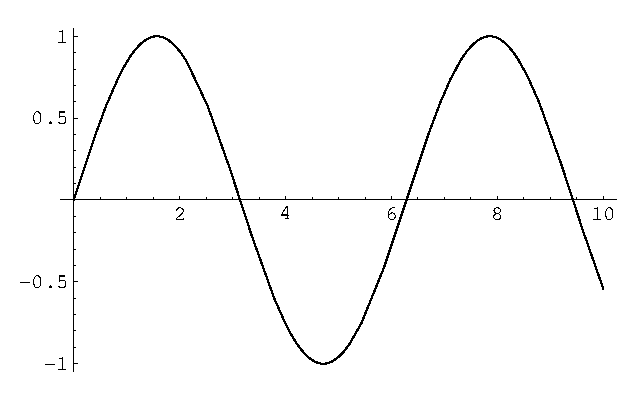
\includegraphics[width=5cm]{figures/mathematica}
\caption{Wykres.}\label{rys:plama}
\end{figure}

\begin{figure}[t]
\centering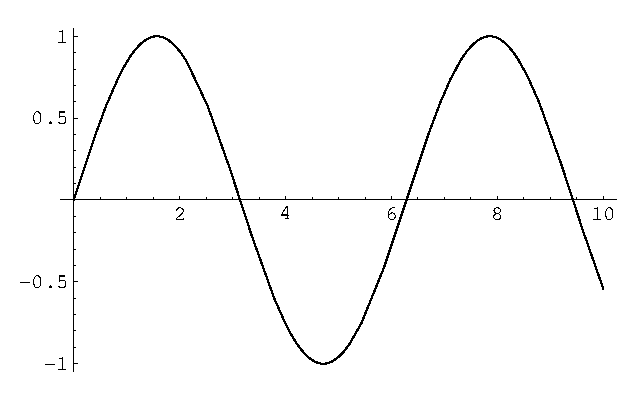
\includegraphics[width=\textwidth]{figures/mathematica}
\fcmfcaption{Ten sam wykres ale na szerokość tekstu. Formatowanie podpisu zgodne z wytycznymi FCMu.}\label{rys:plama2}
\end{figure}

Styl FCMu to nieco inne nagłówki rysunków. Dostepne są one poleceniem \texttt{fcmfcaption} (zob.~rysunek
\ref{rys:plama2}).

\subsection{Tablice}

Tablice to piękna rzecz, choć akurat ich umiejętne tworzenie w \LaTeX{}u nie jest łatwe. 
Jeśli tablica jest skomplikowana, to można ją na przykład wykonać w programie
OpenOffice, a następnie wyeksportować jako plik \akronim{PDF}. W każdym przypadku tablice wstawia się podobnie
jak rysunki, tylko że w środowisko \texttt{table}. Tradycja typograficzna sugeruje umieszczenie opisu tablicy, a więc
elementu \texttt{caption} ponad jej treścią (inaczej niż przy rysunkach).  

Tablica~\ref{tab:tabela} pokazuje pełen przykład.

\begin{table}[ht]
\caption{Przykładowa tabela. Styl opisu jest zgodny z rysunkami.}\label{tab:tabela}
\centering\footnotesize%
\begin{tabular}{l c}
\toprule
artykuł & cena [zł] \\
\midrule
bułka   & $0,4$ \\
masło   & $2,5$ \\
\bottomrule
\end{tabular}
\end{table}

Zasady FCMu sugerują nieco inne nagłówki tablic. Dostepne są one poleceniem \texttt{fcmtcaption} (zob.~tablicę
\ref{tab:tabela2}).

\begin{table}[ht]
\fcmtcaption{Przykładowa tabela. Styl opisu jest zgodny z wytycznymi FCMu.}\label{tab:tabela2}
\centering\footnotesize%
\begin{tabular}{l c}
\toprule
artykuł & cena [zł] \\
\midrule
bułka   & $0,4$ \\
masło   & $2,5$ \\
\bottomrule
\end{tabular}
\end{table}


\subsection{Checklista}

\begin{itemize}
\item Znakiem myślnika jest w LaTeXu dywiz pełen (---) albo półpauza (--), przykład:
  A niech to jasna cholera --- wrzasnąłem.

\item Połączenie między wyrazami to zwykły myślnik, przykład:   północno-zachodni

\item Sprawdź czy tutuł pracy ma maksymalnie dwa wiersze i czy stanowią one pełne frazy
  (czy nie ma przeniesienia bez sensu).

\item Sprawdź ostrzeżenia o 'overfull' i 'underful' boxes. Niektóre z nich można zignorować (spójrz
  na wynik formatowania), niektóre trzeba poprawić; czasem przeformułować zdanie.

item Przypisy stawia się wewnątrz zdań lub za kropką, przykład:
  Footnote is added after a comma.\footnote{Here is a footnote.}

\item Nie używaj przypisów zbyt często. Zobacz, czy nie lepiej będzie zintegrować przypis z tekstem.

\item Tytuły tabel, rysunków powinny kończyć się kropką.

\item Nie używaj modyfikatora [h] (here) do rysunków i tabel. Rysunki i tabele powinny być
  justowane do góry strony lub na stronie osobnej.

\item Wyróżnienie w tekście to polecenie \emph{wyraz}, nie należy używać czcionki pogrubionej (która
  wystaje wizualnie z tekstu i rozprasza).

\item Nazwy plików, katalogów, ścieżek, zmiennych środowiskowych, klas i metod formatujemy poleceniem
  \texttt{plik\_o\_pewnej\_nazwie}.

\item Po ostatniej zmianie do treści, sprawdź i przenieś wiszące spójniki wstawiając przed nie znak
  tyldy (twardej spacji), przykład:
  Ala i~kotek nie lubią mleczka, a~Stasiu lubi.
  
\item Za i.e. (id est) i e.g. (exempli gratia) stawia się zwyczajowo przecinek w typografii amerykańskiej.

\item Przed i za pełną pauza nie ma zwyczajowo spacji w typografii amerykańskiej, przykład:
  Darn, this looks good---said Mary.

\item Zamykający cudzysłów oraz footnote wychodzą za ostatni znak interpunkcji w typografii 
  amerykańskiej, przykłady:
  It can be called a ``curiosity,'' but it's actually normal.
  Footnote is added after a comma.\footnote{Here is a footnote.}

\item Odwołania do tabel i rysunków zawsze z wielkiej litery, przykład:
  In Figure~\ref{rys:plama} we illustrated XXX and in Table~\ref{tab:tabela} we show detailed data.
  
\end{itemize}


\section{Literatura i materiały dodatkowe}

Materiałów jest mnóstwo. Oto parę z nich:
\begin{itemize}
    \item \emph{The Not So Short Introduction\ldots}, która posiada również tłumaczenie 
    w języku polskim.\\
    \url{http://www.ctan.org/tex-archive/info/lshort/english/lshort.pdf}

    \item Klasy stylu \texttt{memoir} posiadają bardzo wiele informacji o składzie tekstów
    anglosaskich oraz sposoby dostosowania \LaTeX{}a do własnych potrzeb.\\
    \url{http://www.ctan.org/tex-archive/macros/latex/contrib/memoir/memman.pdf}
    
    \item Nasza grupa dyskusyjna i repozytorium Git są również dobrym miejscem aby zapytać
    (lub sprawdzić czy pytanie nie zostało już zadane).\\
    \url{https://github.com/politechnika/put-latex}

    \item Dla łaknących więcej wiedzy o systemie LaTeX podstawowym źródłem informacji
    jest książka Lamporta~\cite{Lamport1985}. Prawdziwy \emph{hardcore} to oczywiście
    \emph{The \TeX{}book} profesora Knutha~\cite{Knuth1986}.
\end{itemize}



%--------------------------------------
% Informacja o prawach autorskich
%--------------------------------------

% \ppcolophon

\end{document}
